\documentclass{article}
\usepackage[utf8]{inputenc}

\title{CS224D Assignment1}
\author{Nathan Wan}
\date{April 2016}

\usepackage{natbib}
\usepackage{graphicx}
% for lists
\usepackage{enumerate}
% for fractions
\usepackage{amsmath}
% for special R
\usepackage{amsfonts}

% my macros
% d/dx etc - usage: \dd{\mathbf x} or \dd[J]{\mathbf x}
\newcommand{\dd}[2][]{\frac{\partial #1}{\partial #2}}
% matrix dimentions
\newcommand{\R}[1]{\mathbb{R}^{#1}}

\begin{document}

\maketitle


\section{Softmax}

\begin{enumerate}[(a)]
\item \begin{align*} 
\mathrm{softmax}(\mathbf{x}+c) &= softmax(\mathbf{x}+c)_i \\
&= \frac{e^{x_i+c}}{\sum_j{e^{x_j+c}}} \\
&= \frac{e^{x_i}e^{c}}{\sum_j{e^{x_j}e^{c}}} \\
&= \frac{e^{c}e^{x_i}}{e^{c}\sum_j{e^{x_j}}} \\
&= \frac{e^{x_i}}{\sum_j{e^{x_j}}} \\
&= \mathrm{softmax}(\mathbf{x}) 
\end{align*}

\end{enumerate}


\section{Neural Network Basics}

\begin{enumerate}[(a)]

% (a)
\item $$
\sigma(x) = \frac{1}{1+e^{-x}}
$$
By chain rule:
\begin{align*} 
\frac{d}{dx}\sigma(x) &= \frac{-1}{(1+e^{-x})^2} \frac{d}{dx}(1+e^{-x}) \\
&= \frac{-1}{(1+e^{-x})^2} (-e^{-x}) \\
&= \frac{1}{1+e^{-x}} (\frac{1 + e^{-x} - 1}{1+e^{-x}}) \\
&= \frac{1}{1+e^{-x}} (\frac{1 + e^{-x}}{1+e^{-x}} - \frac{1}{1+e^{-x}})  \\
&= \sigma(x) (1 - \sigma(x))
\end{align*}

% (b)
\item NOTE: Please note that variables $\hat{y}$, $y$, $x$, $\theta$, $h$ and $a$ without subscripts are vectors.

Since $$
\hat{y} = softmax(\mathbf{\theta})
$$ then $$
\hat{y}_i = softmax(\mathbf{\theta})_i = \frac{e^{\theta_i}}{\sum_j{e^{\theta_j}}}
$$
Using division derivative rule:
$$
\frac{\partial}{\partial\theta_{w=i}} softmax(\mathbf{\theta})_i = \frac{(\sum_j{e^{\theta_j}})e^{\theta_i}-(e^{\theta_i})^2}{(\sum_j{e^{\theta_j}})^2} \\
= softmax(\mathbf{\theta})_i - softmax(\mathbf{\theta})_i^2
$$

and

$$
\frac{\partial}{\partial\theta_{w\neq i}} softmax(\mathbf{\theta})_i = \frac{(\sum_j{e^{\theta_j}}) 0-e^{\theta_i}(e^{\theta_w})}{(\sum_j{e^{\theta_j}})^2} \\
= - softmax(\mathbf{\theta})_i softmax(\mathbf{\theta})_w
$$

thus $$
\frac{\partial}{\partial\theta}CE(y,\hat{y}) = \frac{\partial}{\partial\theta}-\sum_i{y_i log(\hat{y}_i)} \\
= -\sum_i{y_i \frac{\partial}{\partial\theta}log(\hat{y}_i)} \\
= -y_k \frac{1}{\hat{y}_k}\frac{\partial}{\partial\theta}\hat{y}_k
$$

since $y_i = 0 : \forall i \neq k$.  For $\theta_{w=k}$ $$
-\frac{1}{\hat{y}_w}\frac{\partial}{\partial\theta}\hat{y}_w =
-\frac{1}{\hat{y}_w}(1 - \hat{y}_w)\hat{y}_w = \hat{y}_w - 1
$$

and for $\theta_{w \neq k}$ $$
-\frac{1}{\hat{y}_w}\frac{\partial}{\partial\theta}\hat{y}_w =
-\frac{1}{\hat{y}_w}(-\hat{y}_k \hat{y}_w) = \hat{y}_w
$$

Since $\mathbf{y}$ is a one-hot vector, $$
\frac{\partial}{\partial\theta}CE(y,\hat{y}) = \hat{y} - y
$$

% (c)
\item Let $\theta = h W_2 + b_2$ so that $$
\hat{y} = softmax(h W_2 + b_2) = softmax(\theta)
$$ and let $a = x W_1 + b_1$ so that $$
h = \sigma(x W_1 + b_1) = \sigma(a)
$$

Also consider for any linear layer $y = xW + b$ in a network, the partial derivative must be $$
\frac{\partial y}{\partial x} = \frac{\partial y}{\partial x} W^T
$$

First, with the input layer $$
\frac{\partial J}{\partial x} = \frac{\partial J}{\partial a} \frac{\partial a}{\partial x} \\
= \frac{\partial J}{\partial a} W_1^T
$$

by chain rule and since the partial is applied element-wise $$
\frac{\partial J}{\partial a} =  \frac{\partial h}{\partial a} \frac{\partial J}{\partial h} \\
= \left ( h(h-1) \circ \dd[J]{h} \right )
$$

but is equivalent to a square matrix with those values along the diagonal.  Since $h$ is a linear transformation of $\theta$

$$
\dd[J]{h} = \dd[J]{\theta} \dd[\theta]{h} \\
= \dd[J]{\theta} W_2^T
$$

And as seen from the previous section, $\frac{\partial J}{\partial\theta} = \frac{\partial}{\partial\theta}CE(y,\hat{y}) = \hat{y} - y$. When put together, $$
\dd[J]{x} = \left ( h(h-1) \circ (\hat{y} - y) W_2^T \right ) W_1^T
$$

Also note that dimensions check out:
$$
\R{1 \times D_x} = \left ( \R{1 \times H} \circ (\R{1 \times D_y}) \R{D_y \times H} \right ) \R{H \times D_x}
$$

% (d)
\item Between the input and hidden layer, there is a linear transformation of $D_x$ input units and a bias term for $h$ hidden layer units,

$$ (D_x + 1) \times H $$

and similarly between the hidden and output layers,

$$ (H + 1) \times D_y $$.  Total parameters is the sum of those two quantities.

$$ (D_x + 1) H + (H + 1) D_y $$

\end{enumerate}


\section{word2vec}

\begin{enumerate}[(a)]

% (a)
\item It is given $$
\hat{y}_o = \frac{exp(u_o^T v_c)}{\sum_{w}exp(u_w^T v_c)}
$$ and that $u_i : i \in |U|$ and $v_o$ are column vectors.

\begin{align*} 
\dd{v_c}J_{sm} &= \dd{v_c} -log(\hat{y}_o) \\
&= -\dd{v_c}u_o^T v_c + \frac{\sum_{w}exp(u_w^T v_c)\dd{v_c}u_w^T v_c}{\sum_{w}exp(u_w^T v_c)} \\
&= -u_o + \sum_{w}\hat{y}_w u_w
\end{align*}

% (b)
\item

\begin{align*} 
\dd{u_i}J_{sm} &= \dd{u_i} -log(\hat{y}_o) \\
&= -\dd{u_i}u_o^T v_c + \frac{\sum_{w}exp(u_w^T v_c)\dd{u_i}u_w^T v_c}{\sum_{w}exp(u_w^T v_c)} \\
&= -\dd{u_i}u_o^T v_c + \sum_{w} \hat{y} \dd{u_i}u_w^T v_c
\end{align*}

Let's distinguish between $i = o$ and $i \neq o$. $$
\dd{u_{i=o}}J_{sm} = -v_c + \hat{y}_i v_c \\
= (\hat{y}_i - 1)v_c
$$ $$
\dd{u_{i \neq o}}J_{sm} = \hat{y}_i v_c
$$

and so $$
\dd{U}J_{sm} = v_c * (\hat{y} - y)
$$

where $U \in \R{d \times V}$, $v_c \in \R{d \times 1}$ and $(\hat{y} - y) \in \R{1 \times V}$.

% (c)
\item Given $$
J_{ns} = -log(\sigma(u_o^T v_c)) - \sum_k log(\sigma(-u_k^T v_c))
$$ and that $$
\dd{x} log(\sigma(x)) = \frac{1}{\sigma(x)}(1-\sigma(x))\sigma(x) = 1 - \sigma(x)
$$ and that $$
\sigma(-x) = 1 - \sigma(x)
$$

we see that 

\begin{align*} 
\dd{v_c}J_{ns} &= -(1 - \sigma(u_o^T v_c))u_o - \sum_k (1 - \sigma(-u_k^T v_c))(-u_k) \\ 
&= -(1 - \sigma(u_o^T v_c))u_o + \sum_k \sigma(u_k^T v_c)u_k
\end{align*}

and

\begin{align*} 
\dd{u_{i=o}}J_{ns} &= -(1 - \sigma(u_o^T v_c))v_c \\ 
\dd{u_{i \in K}}J_{ns} &= -(1 - \sigma(-u_k^T v_c))(-v_c) \\
&= \sigma(u_k^T v_c) v_c
\end{align*}

This cost function is more efficient to compute because there is no summation over the entire vocabulary of $|U|$, instead, we only look at $K$ samples so the computation speed up is on the order of $\frac{O(|U|)}{O(K)}$.

% (d)
\item For Skipgram: $$
\dd{v_c}J_{sg} = \sum_{-m \leq j \leq m,j \neq 0} \dd{v_c}F(u_{c+j}, v_c)
$$ and $$
\dd{U}J_{sg} = \sum_{-m \leq j \leq m,j \neq 0} \dd{U}F(u_{c+j}, v_c)
$$

For CBOW, note that since the center word is an output vector: $$
\dd{U}J_{CBOW} = \dd{U} F(u_c,\hat{v})
$$

and for $j \in \{ -m \leq j \leq m,j \neq 0 \}$, $$
\dd{v_j}F(u_c, \hat{v}) = \dd[F]{\hat{v}} \dd[\hat{v}]{v_j} \\
= \dd{\hat{v}} F(u_c, \hat{v})
$$

\setcounter{enumi}{6}
% (g)
\item Some stop words, like "a" and "the" are clearly separate from the other words; "an" is also a stop word, but probably there wasn't enough examples for it to be distinguished.  Similarly, only some more frequent punctuation like "?" are distinguishable.  The adjectives are grouped in a very distinct shape, but it's difficult to glean something significant from the words within the shape.

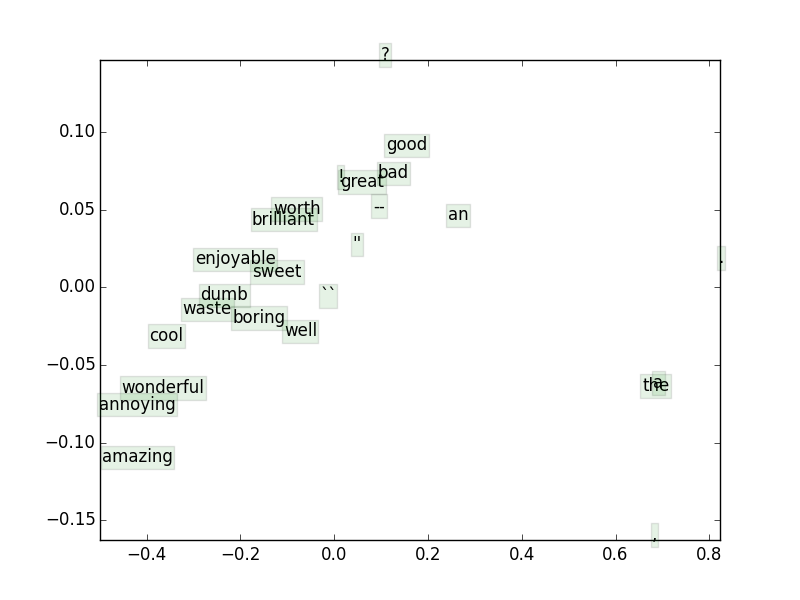
\includegraphics[width=\textwidth]{q3_word_vectors}


\end{enumerate}


\section{Sentiment Analysis}

\begin{enumerate}[(a)]

\setcounter{enumi}{1}
% (b)
\item Regularization keep the model parameters from overfitting training data.  

% (c)
\item I selected the regularization value that maximized dev accuracy.  I first swept values from $10^{-10}$ to $10^{0}$ before narrowing in on the $10^{-4}$ region.  Despite a step of $log(.2)$, the best value was still $10^{-4}$:

\iffalse
=== Recap ===
Reg     Train       Dev
1.000000E-10    29.892322   30.245232
1.000000E-09    29.892322   30.245232
1.000000E-08    29.892322   30.245232
1.000000E-07    29.892322   30.245232
1.000000E-06    29.892322   30.154405
1.000000E-05    29.798689   30.154405
1.000000E-04    29.658240   30.790191
1.000000E-03    27.317416   25.431426
1.000000E-02    27.247191   25.522252
1.000000E-01    27.247191   25.522252
1.000000E+00    12.816011   12.806540

Best regularization value: 1.000000E-06
Test accuracy (%): 28.144796

=== Recap ===
Reg     Train       Dev
1.000000E-05    29.798689   30.154405
1.584893E-05    29.786985   30.245232
2.511886E-05    29.822097   30.063579
3.981072E-05    29.857210   30.063579
6.309573E-05    29.763577   30.154405
1.000000E-04    29.658240   30.790191
1.584893E-04    29.412453   29.609446
2.511886E-04    28.710206   28.337875
3.981072E-04    28.113296   26.521344
6.309573E-04    27.516386   25.794732

Best regularization value: 1.000000E-04
Test accuracy (%): 27.285068
\fi

\begin{tabular}{| l | l |}
  \hline
  Train & 29.658240 \\
  Dev   & 30.790191 \\
  Test  & 27.285068 \\
  \hline
\end{tabular}

Oddly, by accident I tested $10^{-6}$ and I actually got a test accuracy of $28.1$, which suggests we should have a stronger bias towards lower regularization values.

% (d)
\item As we increase the regularization factor, we see a small increase in accuracy until about $10^{-4}$.  After which, regularization will keep the model from correctly learning features in the data.

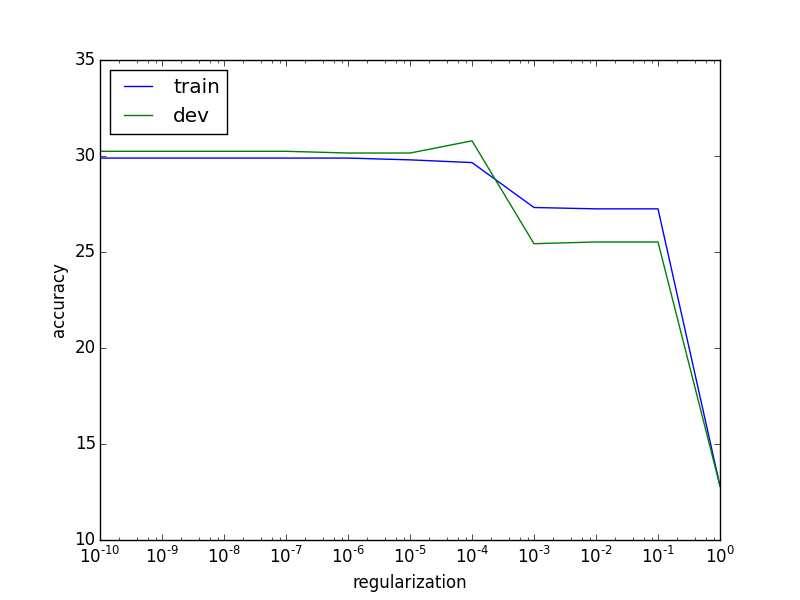
\includegraphics[width=\textwidth]{q4_reg_v_acc_001}
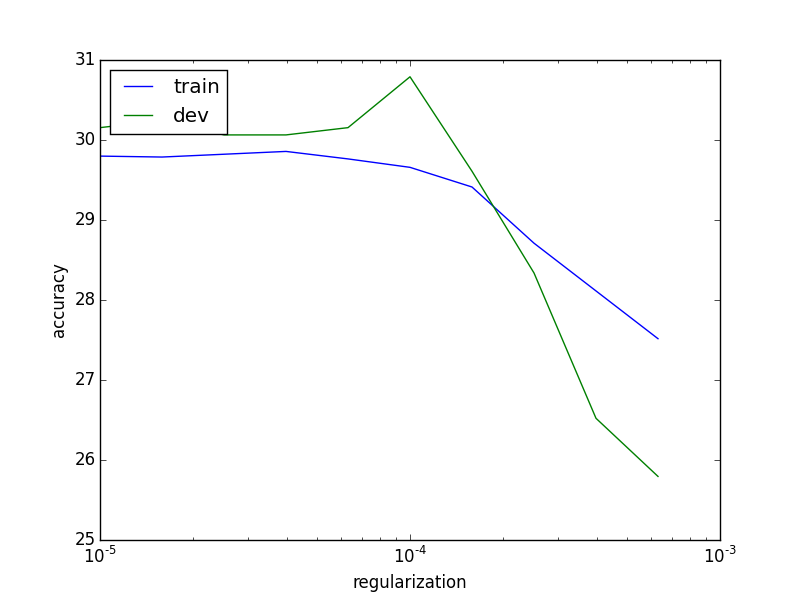
\includegraphics[width=\textwidth]{q4_reg_v_acc}

\end{enumerate}

\end{document}
